\section{Object Sets and ISOD Analysis}\label{app:objects}
\begin{figure}[H]
\centering
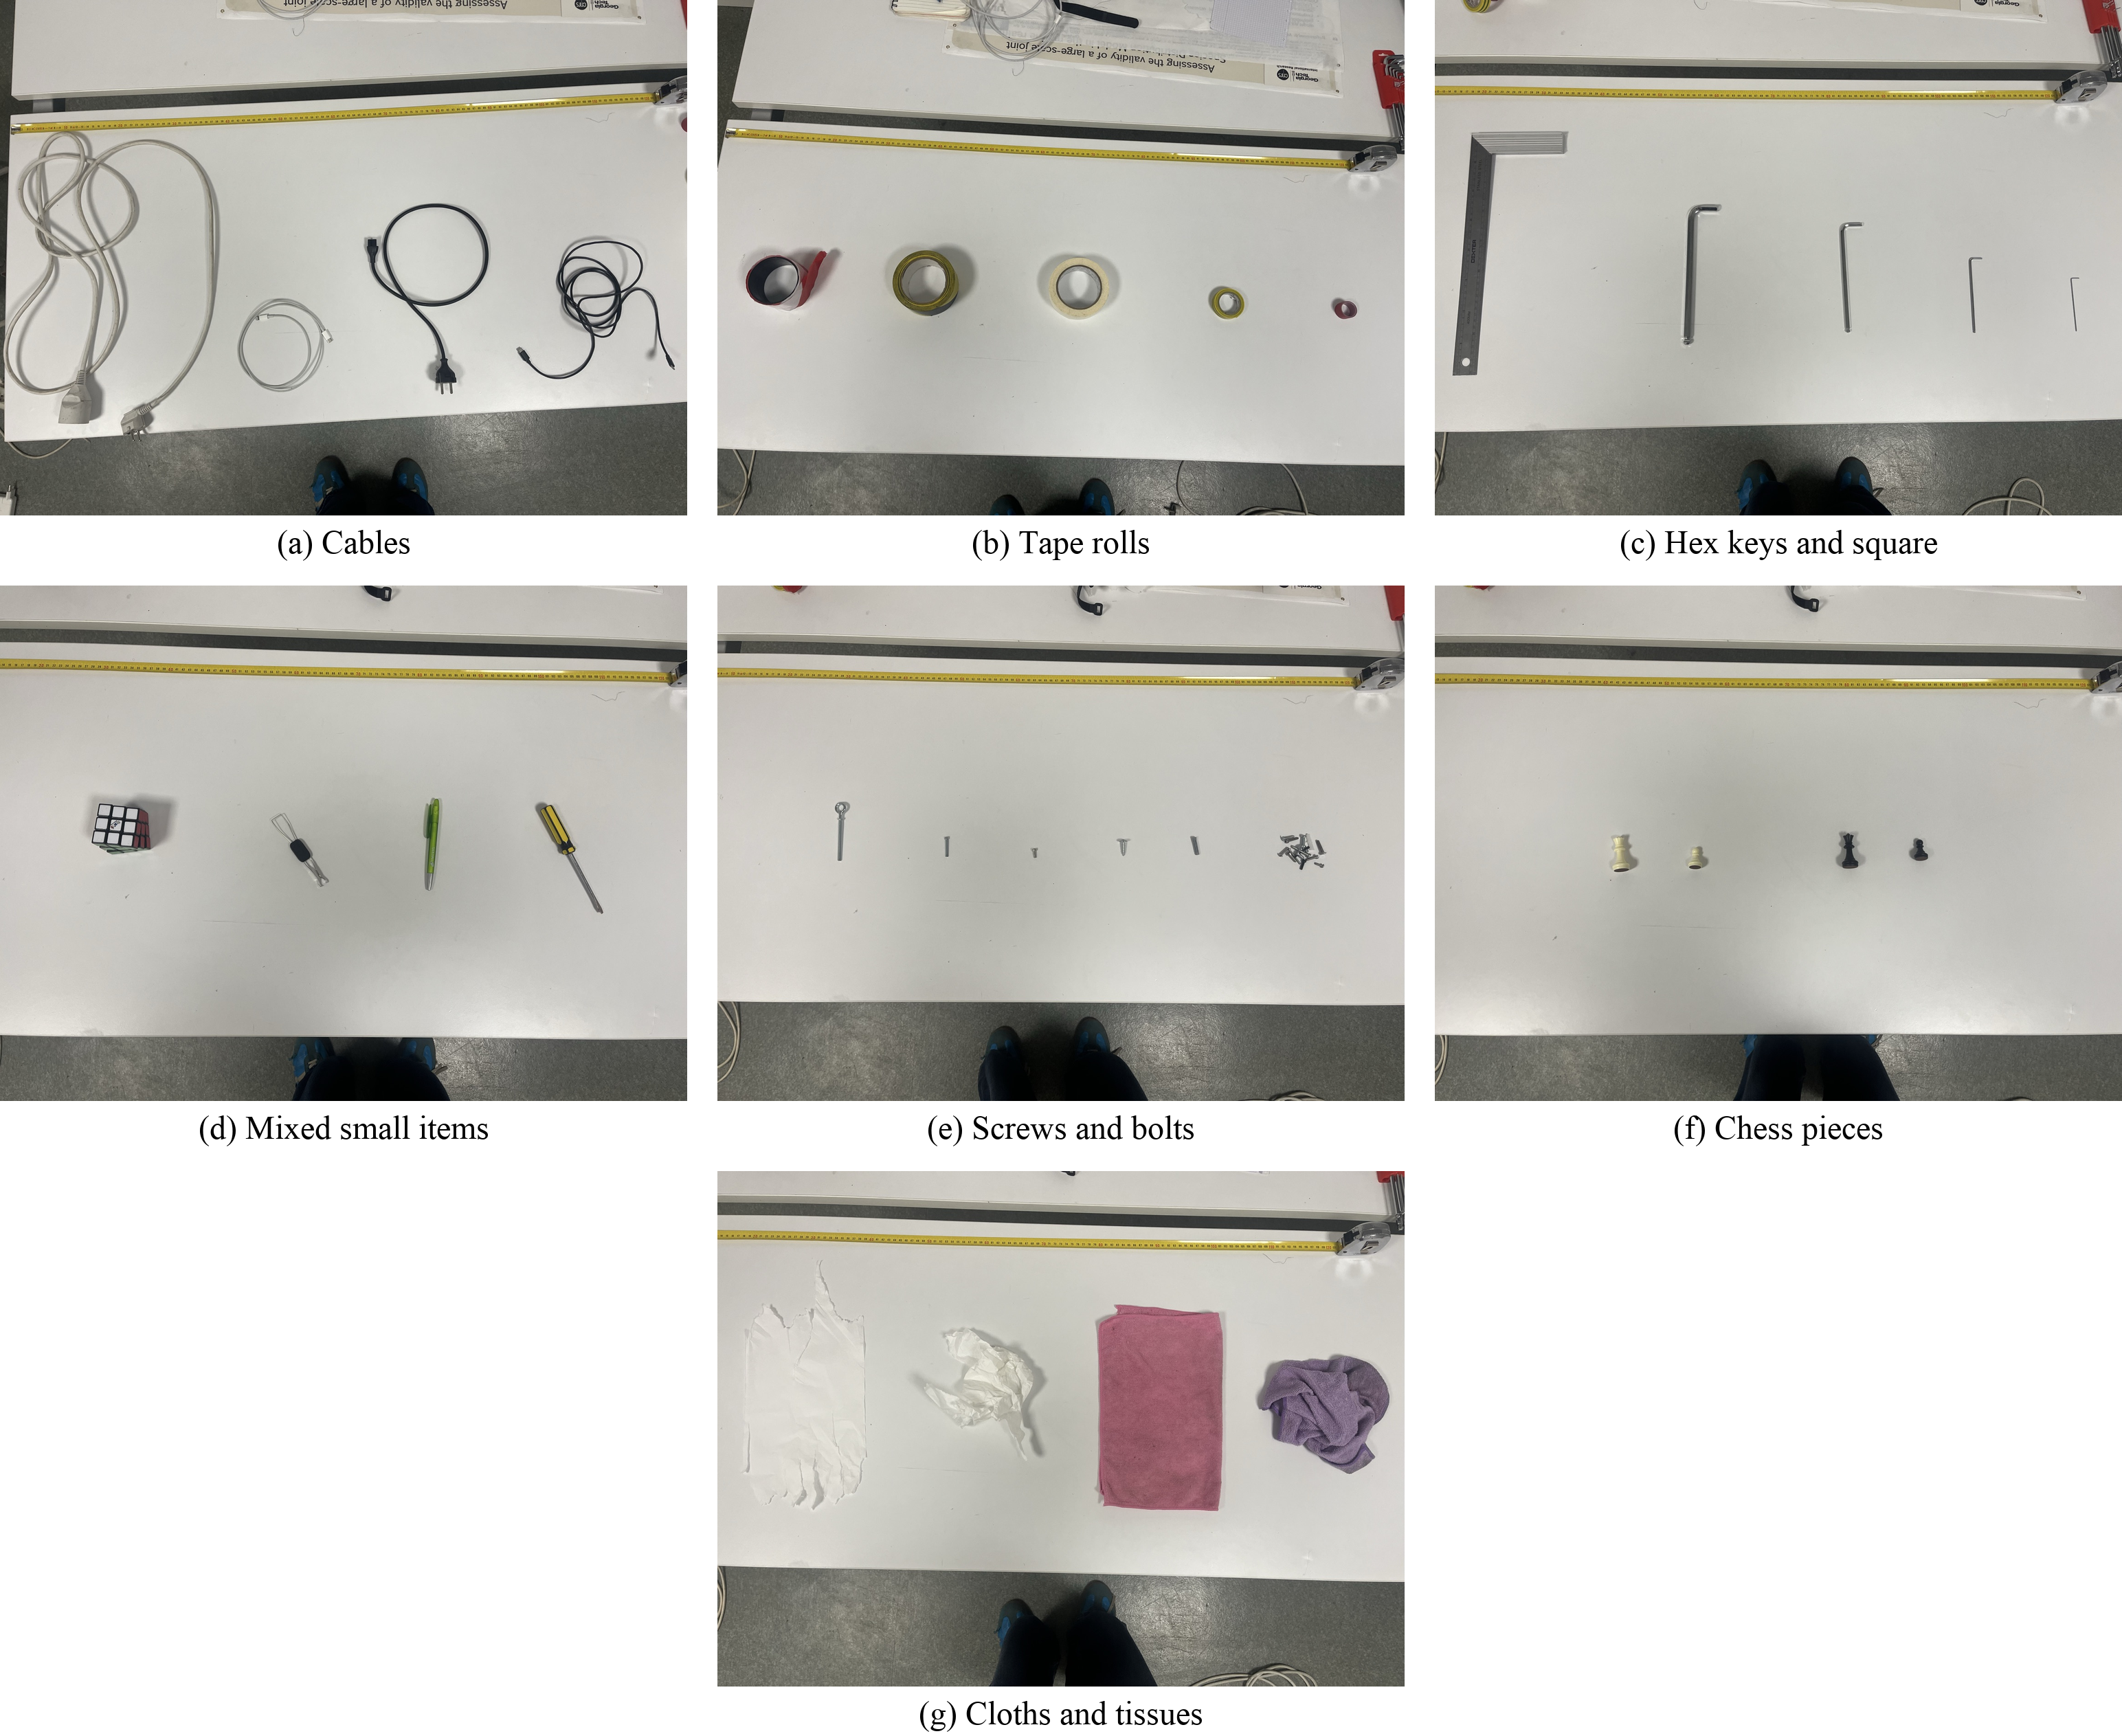
\includegraphics[width=\textwidth,height=0.51\textheight,keepaspectratio]{figures/object_sets.png}
\caption{GTE-Floor's seven object sets. Cables, hex keys and screws provide thin or small obstacles; cloths and tissues include flat and crumpled forms. Tape rolls and chess pieces provide taller objects, while the mixed set adds everyday items.}
\label{fig:objects}
\end{figure}

Figure~\ref{fig:isod-scale} extends the size and range analysis to all
300 ISOD test frames. Here, each connected region of the reference mask
is an approximate object: touching objects can merge and one object can
split into fragments. These are not verified SAM instance labels.
\begin{figure}[H]
\centering
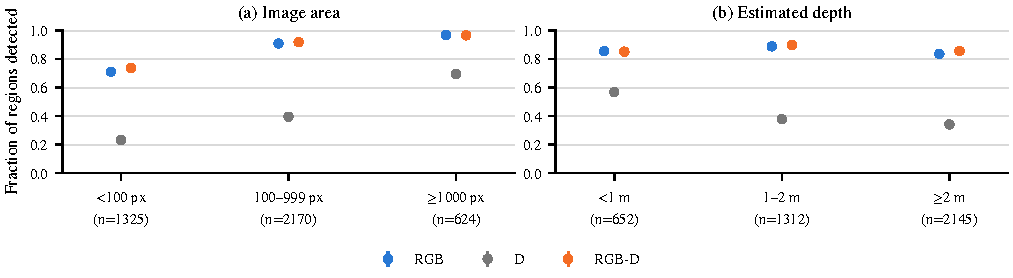
\includegraphics[width=\textwidth]{figures/isod_distance_size.pdf}
\caption{Reference-trained ESANet on ISOD by mask-region area and estimated depth: three-seed means and standard deviations. $n$: regions across frames, not unique physical objects. Depth is the median positive reading inside each region; ten regions with fewer than half valid depth pixels are excluded from (b). Thin-object depth can measure the floor.}
\label{fig:isod-scale}
\end{figure}

\clearpage
\section{Experimental Configuration and Label Construction}\label{app:configuration}

Table~\ref{tab:experiment-matrix} summarizes the training runs.
All learned models use 1,400 ISOD training images and 300 validation
images. We train each model using either the reference obstacle masks
prepared from ISOD annotations or masks generated automatically by
SAM~3 from RGB images. Both use the same model architecture, training
images and validation masks.

\begin{table}[H]
\caption{Training configurations.}
\label{tab:experiment-matrix}
\centering\small
\begin{tabular}{llllrr}
\toprule
Model & Input & Training labels & Label sources & Epochs/run & \shortstack{Seeds per\\label source}\\
\midrule
ESANet & RGB & Binary pixel mask & Reference, SAM & 500 & 3\\
ESANet & D & Binary pixel mask & Reference, SAM & 500 & 3\\
ESANet & RGB-D & Binary pixel mask & Reference, SAM & 500 & 3\\
U-Net/MobileNetV2 & RGB & Binary pixel mask & Reference, SAM & 15 & 3\\
YOLOv8n-seg & RGB & Instance masks and boxes & Reference, SAM & 60 & 3\\
YOLOv8n detector & RGB & Object boxes & Reference, SAM & 60 & 3\\
\bottomrule
\end{tabular}
\end{table}

YOLOv8n-seg uses polygons from binary masks, omitting contours below
20 pixels. The box detector uses separate object IDs, including one box
for disconnected visible parts of the same object. Unresolved piles
remain groups.

\textbf{Reference labels.} We use SAM to identify objects within ISOD's
not-drivable mask, then apply floor-contact and connected-region rules
to exclude walls and furniture. The segmentation training set has
70 masks checked by hand and 1,330 automatically prepared masks; the
box-detector set has 85 and 1,315. All 300 validation masks were checked.
Of the 300 test masks, 30 were checked by hand, ten per location. On
those frames, the automatically prepared masks have pixel IoU 0.929
against the corrected masks.

\textbf{Automatic generation.} SAM 3 weights are frozen. Full RGB images
are processed with exactly these three prompts:
\begin{quote}
small object on the floor\\
cable on the floor\\
things on the floor
\end{quote}
Confidence is 0.6 and mask threshold 0.5. Duplicate masks are merged;
unresolved piles remain groups. We chose prompts on 30 reviewed training
frames and checked alternatives on 300 validation frames. Generating
labels uses only RGB images, without ISOD masks or manual corrections.
The SAM~3 checkpoint is \textnormal{bodhicitta/sam3}.

\textbf{Training settings.} ESANet uses 640$\times$448 inputs, batch 8,
SGD (learning rate 0.01, momentum 0.9, weight decay $10^{-4}$), OneCycle
scheduling and median-frequency class weights. U-Net uses batch 8 and
AdamW (learning rate $3\times10^{-4}$), with binary cross-entropy plus
soft Dice loss. YOLOv8n-seg uses AdamW (learning rate 0.002, no warm-up
bias rate) and linear learning-rate decay, with mosaic disabled for the
last ten epochs. The box detector uses COCO initialization, 640-pixel
inputs, batch 16, SGD (learning rate 0.01, momentum 0.937, weight decay
$5\times10^{-4}$) and linear decay. Box inference uses confidence 0.25
and NMS IoU 0.7. YOLOv8n-seg checkpoints are checked every five epochs;
selection criteria are in Table~\ref{tab:models}.

\textbf{Inference speed.} Table~\ref{tab:inference-cost} measures single-image
latency including preprocessing, inference and transfer to CPU, after
warm-up (three CPU passes, 15 GPU passes). CPU uses float32; GPU uses
float16 for YOLO and bfloat16 for SAM. SAM shares image features across
its three prompts. These are server measurements, not on-robot timings.

\begin{table}[H]
\caption{End-to-end latency (ms).}\label{tab:inference-cost}
\centering\small
\begin{tabular}{lrr}
\toprule Hardware & YOLOv8n boxes & SAM 3 (three prompts)\\\midrule
Xeon Gold 6230, 8 threads & \textbf{33.86} & 13263.34\\
H200 MIG (71 GiB) & \textbf{4.04} & 183.14\\
\bottomrule\end{tabular}
\end{table}


\clearpage
\section{Evaluation and Per-Item Results}\label{app:evaluation}

Object recall counts an object when predictions together cover at least
half its pixels. Component F1 uses SegmentMeIfYouCan's adjusted overlap
and precision~\cite{chan2021segment}: splits and merges are allowed, but
background between objects lowers precision. We average its 11
thresholds from 0.25 to 0.75; false regions have precision below 0.5.
Boxes above confidence 0.25 are filled and united for this comparison.
Native box AP uses one-to-one matching and therefore penalizes different
groupings (reference/SAM AP50: 0.599/0.630; AP50:95: 0.407/0.445).

ISOD objects are connected regions of the reference masks; GTE-Floor
uses annotated item/group IDs, including disconnected visible parts.
There are 262 object/recording pairs and 1,310 object/frame observations.
Bootstrap intervals resample 64 recordings, keeping each recording's
five frames together. Table~\ref{tab:full-scores} gives seed variation
and Table~\ref{tab:per-item} gives per-item recall.

\begin{longtable}{llrrrr}
\caption{All scores with training-seed standard deviation.}\label{tab:full-scores}\\
\toprule Dataset & Method & Pixel IoU & Object recall & Component F1 & False regions/frame\\\midrule\endfirsthead
\toprule Dataset & Method & Pixel IoU & Object recall & Component F1 & False regions/frame\\\midrule\endhead
ISOD & ESANet RGB, ref. & 0.711$\pm$0.009 & 0.854$\pm$0.008 & 0.591$\pm$0.024 & 3.19$\pm$0.45\\
ISOD & ESANet D, ref. & 0.318$\pm$0.009 & 0.388$\pm$0.017 & 0.131$\pm$0.005 & 5.97$\pm$0.53\\
ISOD & ESANet RGB-D, ref. & 0.708$\pm$0.005 & 0.867$\pm$0.007 & 0.583$\pm$0.012 & 3.63$\pm$0.16\\
ISOD & U-Net RGB, ref. & 0.724$\pm$0.008 & 0.750$\pm$0.019 & 0.693$\pm$0.012 & 2.03$\pm$0.24\\
ISOD & YOLOv8n-seg RGB, ref. & 0.725$\pm$0.010 & 0.751$\pm$0.011 & 0.735$\pm$0.008 & 1.13$\pm$0.28\\
ISOD & YOLOv8n boxes RGB, ref. & 0.498$\pm$0.011 & 0.806$\pm$0.003 & 0.501$\pm$0.019 & 3.88$\pm$0.30\\
ISOD & ESANet RGB, SAM & 0.689$\pm$0.009 & 0.870$\pm$0.004 & 0.566$\pm$0.010 & 4.84$\pm$0.09\\
ISOD & ESANet D, SAM & 0.304$\pm$0.019 & 0.388$\pm$0.026 & 0.121$\pm$0.011 & 6.16$\pm$0.39\\
ISOD & ESANet RGB-D, SAM & 0.680$\pm$0.017 & 0.883$\pm$0.004 & 0.543$\pm$0.021 & 5.75$\pm$0.71\\
ISOD & YOLOv8n boxes RGB, SAM & 0.522$\pm$0.012 & 0.802$\pm$0.010 & 0.517$\pm$0.009 & 3.88$\pm$0.03\\
ISOD & SAM 3, three prompts & 0.730 & 0.838 & 0.829 & 1.51\\
ISOD & Floor-plane fit (D) & 0.061 & 0.486 & 0.006 & 151.64\\
\midrule
GTE & ESANet RGB, ref. & 0.486$\pm$0.075 & 0.628$\pm$0.005 & 0.356$\pm$0.034 & 3.65$\pm$0.76\\
GTE & ESANet D, ref. & 0.141$\pm$0.012 & 0.383$\pm$0.011 & 0.067$\pm$0.005 & 8.24$\pm$1.35\\
GTE & ESANet RGB-D, ref. & 0.554$\pm$0.088 & 0.643$\pm$0.062 & 0.428$\pm$0.049 & 2.84$\pm$0.60\\
GTE & U-Net RGB, ref. & 0.487$\pm$0.064 & 0.464$\pm$0.055 & 0.388$\pm$0.032 & 2.40$\pm$0.06\\
GTE & YOLOv8n-seg RGB, ref. & 0.450$\pm$0.023 & 0.600$\pm$0.008 & 0.522$\pm$0.020 & 0.96$\pm$0.12\\
GTE & YOLOv8n boxes RGB, ref. & -- & 0.675$\pm$0.048 & 0.380$\pm$0.024 & 1.29$\pm$0.04\\
GTE & ESANet RGB, SAM & 0.469$\pm$0.021 & 0.781$\pm$0.060 & 0.346$\pm$0.027 & 6.42$\pm$1.31\\
GTE & ESANet D, SAM & 0.126$\pm$0.018 & 0.363$\pm$0.021 & 0.060$\pm$0.012 & 8.82$\pm$1.42\\
GTE & ESANet RGB-D, SAM & 0.498$\pm$0.037 & 0.753$\pm$0.034 & 0.356$\pm$0.029 & 6.03$\pm$0.79\\
GTE & YOLOv8n boxes RGB, SAM & -- & 0.720$\pm$0.005 & 0.393$\pm$0.008 & 1.51$\pm$0.13\\
GTE & SAM 3, three prompts & 0.418 & 0.945 & 0.673 & 2.54\\
GTE & Floor-plane fit (D) & 0.038 & 0.695 & 0.002 & 344.02\\
GTE & RGB-D, depth removed & 0.147$\pm$0.033 & 0.078$\pm$0.025 & 0.084$\pm$0.024 & 2.25$\pm$2.12\\
GTE & RGB-D, other scene's depth & 0.547$\pm$0.104 & 0.641$\pm$0.065 & 0.422$\pm$0.051 & 2.89$\pm$0.69\\
\bottomrule\end{longtable}

\label{app:fullscores}

\textbf{Reference checks and object size.} A check of 14 previously
unreviewed training frames gives pixel IoU 0.912; two frames contain
major errors. This does not verify individual object IDs. Image area is
foreground pixels (GTE-Floor: 640$\times$362; ISOD: 640$\times$422). Floor-distance marks are
not per-object range; unreliable thin-object depth and missing ISOD
calibration prevent physical size estimates.

\begin{table}[H]
\caption{Recovery by annotated GTE-Floor item.}\label{tab:per-item}
\centering\footnotesize
\setlength{\tabcolsep}{3pt}
\begin{minipage}[t]{.49\textwidth}\centering
\begin{tabular}{lrrrr}
\toprule Item & $n$ & RGB & D & RGB-D\\\midrule
black mains lead & 12 & \textbf{0.900} & 0.394 & 0.844\\
black USB lead & 12 & \textbf{0.944} & 0.367 & \textbf{0.944}\\
white extension lead & 12 & 0.800 & 0.272 & \textbf{0.878}\\
white USB-C lead & 12 & \textbf{0.478} & 0.283 & 0.472\\
black pawn & 12 & 0.678 & 0.417 & \textbf{0.761}\\
black queen & 12 & \textbf{0.800} & 0.633 & 0.728\\
white pawn & 12 & \textbf{0.611} & 0.494 & \textbf{0.611}\\
white queen & 12 & 0.644 & 0.406 & \textbf{0.722}\\
large hex key & 6 & 0.678 & 0.144 & \textbf{0.756}\\
medium hex key & 6 & \textbf{0.233} & 0.100 & 0.156\\
small hex key & 6 & \textbf{0.044} & 0.011 & 0.000\\
carpenter's square & 6 & 0.000 & 0.000 & \textbf{0.178}\\
tiny hex key & 5 & 0.000 & \textbf{0.027} & 0.000\\
folded pink cloth & 12 & 0.833 & 0.206 & \textbf{0.922}\\
bundled purple cloth & 12 & 0.889 & 0.917 & \textbf{0.950}\\
\bottomrule\end{tabular}\end{minipage}\hfill
\begin{minipage}[t]{.49\textwidth}\centering
\begin{tabular}{lrrrr}
\toprule Item & $n$ & RGB & D & RGB-D\\\midrule
crumpled tissue & 12 & 0.644 & \textbf{0.978} & 0.767\\
flat paper towel & 12 & 0.439 & 0.217 & \textbf{0.467}\\
Rubik's cube & 6 & 0.889 & 0.789 & \textbf{1.000}\\
wire keycap puller & 6 & \textbf{0.778} & 0.067 & 0.400\\
green ballpoint pen & 6 & \textbf{0.889} & 0.078 & 0.833\\
yellow screwdriver & 6 & \textbf{1.000} & 0.600 & 0.989\\
big screw (eye bolt) & 6 & 0.144 & 0.078 & \textbf{0.311}\\
pile of screws & 6 & \textbf{0.778} & 0.211 & 0.556\\
small screws & 24 & 0.006 & \textbf{0.072} & 0.022\\
white masking roll & 6 & 0.833 & \textbf{0.889} & 0.833\\
tiny red roll & 5 & \textbf{1.000} & 0.360 & \textbf{1.000}\\
red/white striped roll & 6 & \textbf{1.000} & 0.733 & \textbf{1.000}\\
yellow/black striped roll & 6 & \textbf{1.000} & 0.978 & \textbf{1.000}\\
small yellow/black roll & 6 & \textbf{1.000} & 0.256 & \textbf{1.000}\\
\bottomrule\end{tabular}\end{minipage}
\par\smallskip{\footnotesize Reference-trained ESANet; $n$: object/recording pairs. Bold: highest recall for each item.}
\end{table}


\clearpage
\section{Training and Validation Curves}\label{app:curves}

Figure~\ref{fig:esanet-curves} shows ESANet optimization and validation.
Training loss decreases while validation loss later increases, most
strongly for depth-only input. Evaluation uses the checkpoint with the
highest validation obstacle IoU.
\begin{figure}[H]
\centering
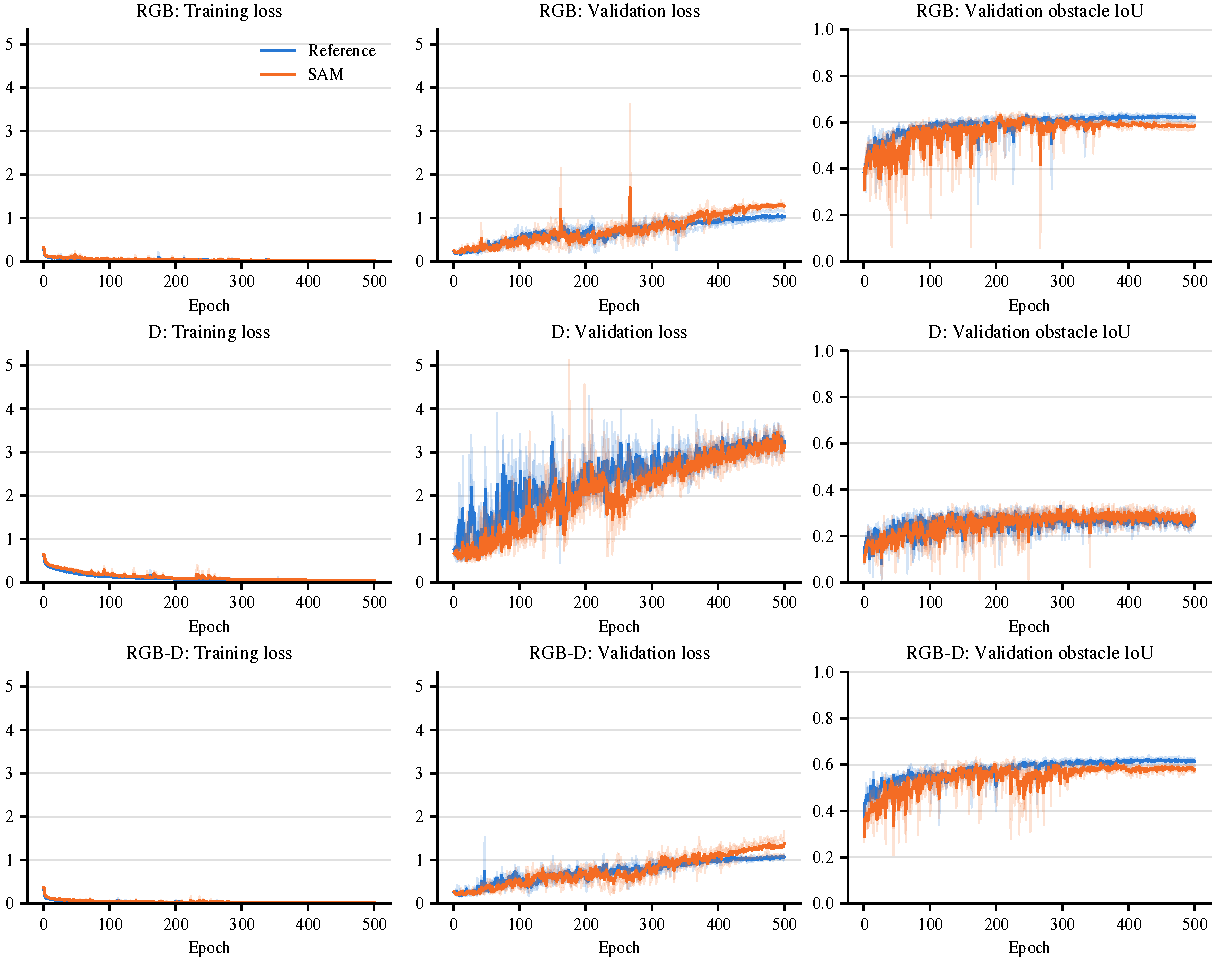
\includegraphics[width=\textwidth]{figures/appendix_esanet_curves.pdf}
\caption{ESANet training and validation. Blue: reference labels; orange: SAM labels. Faint curves are individual runs; bold curves are means. Markers identify the selected checkpoint: circles, triangles and squares for seeds 0, 1 and 2. Epochs and validation scores are in Table~\ref{tab:checkpoints}.}
\label{fig:esanet-curves}
\end{figure}
\begin{table}[H]
\caption{Selected checkpoints.}\label{tab:checkpoints}
\centering\footnotesize
\setlength{\tabcolsep}{5pt}
\begin{tabular}{lrrrrrr}
\toprule
 & \multicolumn{3}{c}{Reference labels} & \multicolumn{3}{c}{SAM labels}\\
\cmidrule(lr){2-4}\cmidrule(lr){5-7}
Model & Seed 0 & Seed 1 & Seed 2 & Seed 0 & Seed 1 & Seed 2\\\midrule
ESANet RGB & 413 / 0.642 & 362 / 0.644 & 181 / 0.627 & 240 / 0.635 & 235 / 0.647 & 200 / 0.643\\
ESANet D & 187 / 0.334 & 292 / 0.331 & 297 / 0.328 & 297 / 0.349 & 331 / 0.331 & 157 / 0.341\\
ESANet RGB-D & 358 / 0.633 & 449 / 0.619 & 431 / 0.641 & 333 / 0.621 & 280 / 0.615 & 227 / 0.634\\
U-Net & 8 / 0.677 & 12 / 0.664 & 15 / 0.666 & 11 / 0.603 & 8 / 0.614 & 4 / 0.594\\
YOLOv8n-seg & 46 / 0.669 & 56 / 0.641 & 51 / 0.653 & 46 / 0.619 & 46 / 0.618 & 41 / 0.594\\
YOLOv8n boxes & 40 / 0.456 & 50 / 0.457 & 45 / 0.456 & 50 / 0.480 & 50 / 0.476 & 60 / 0.474\\
\bottomrule\end{tabular}
\par\smallskip{\footnotesize Cells: epoch / validation obstacle IoU; the box detector uses validation fitness.}
\end{table}


\clearpage
Figures~\ref{fig:baseline-curves} and~\ref{fig:native-curves} show the
remaining RGB models.
\begin{figure}[H]
\centering
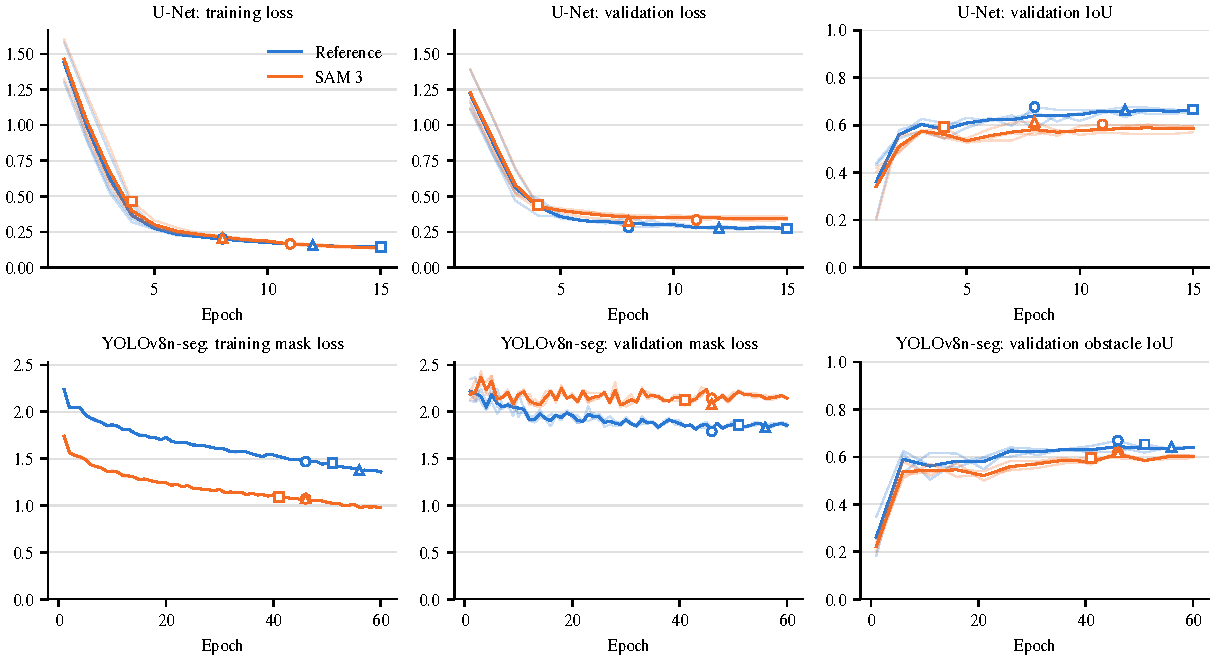
\includegraphics[width=0.9\textwidth]{figures/appendix_rgb_baseline_curves.pdf}
\caption{U-Net and YOLOv8n-seg training and validation. Colors, lines and checkpoint markers follow Fig.~\ref{fig:esanet-curves}. Checkpoints maximize validation obstacle IoU, checked every epoch for U-Net and every five epochs for YOLOv8n-seg.}
\label{fig:baseline-curves}
\end{figure}
\begin{figure}[H]
\centering
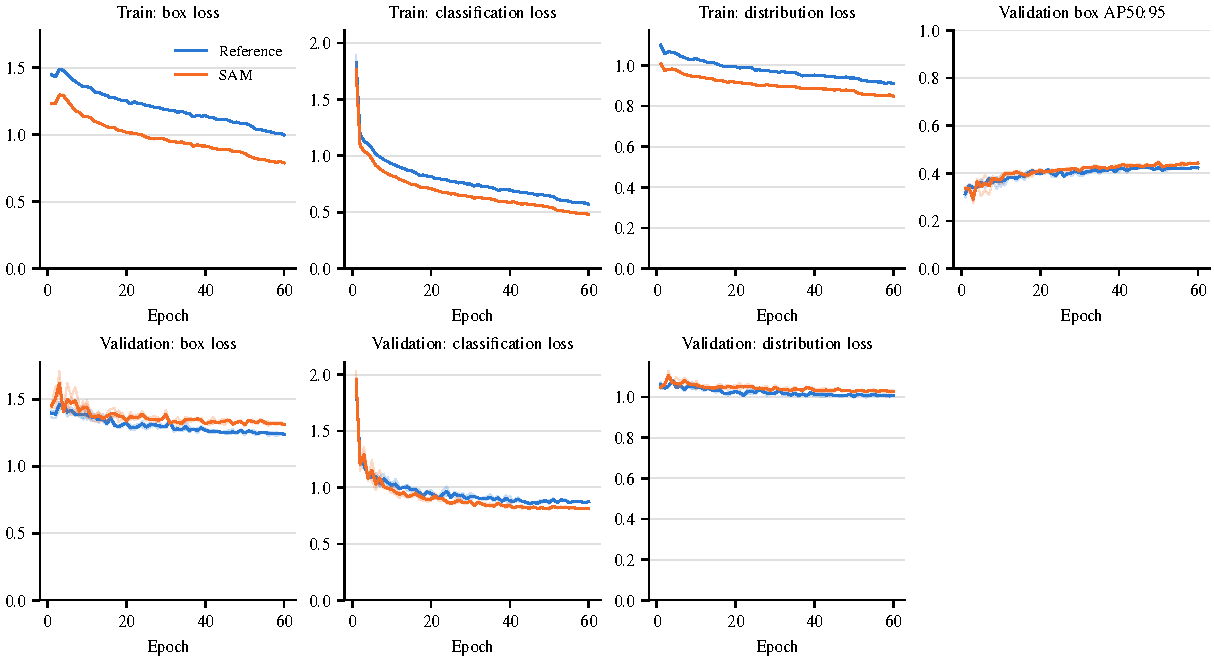
\includegraphics[width=0.9\textwidth]{figures/appendix_native_curves.pdf}
\caption{YOLOv8n box-detector losses and validation AP50:95. Colors, lines and checkpoint markers follow Fig.~\ref{fig:esanet-curves}. Selected checkpoints maximize validation fitness (Table~\ref{tab:checkpoints}).}
\label{fig:native-curves}
\end{figure}

\clearpage
\section{Automatic-Label Examples}\label{app:teacher}

Figure~\ref{fig:teacher-devval} shows the automatic SAM~3 labels used for training next to the reviewed
references. Their pooled mask
IoU is 0.775 on the 30 prompt-development frames, 0.604 on the 300
validation frames and 0.730 on the 300 test frames.
\begin{figure}[H]
\centering
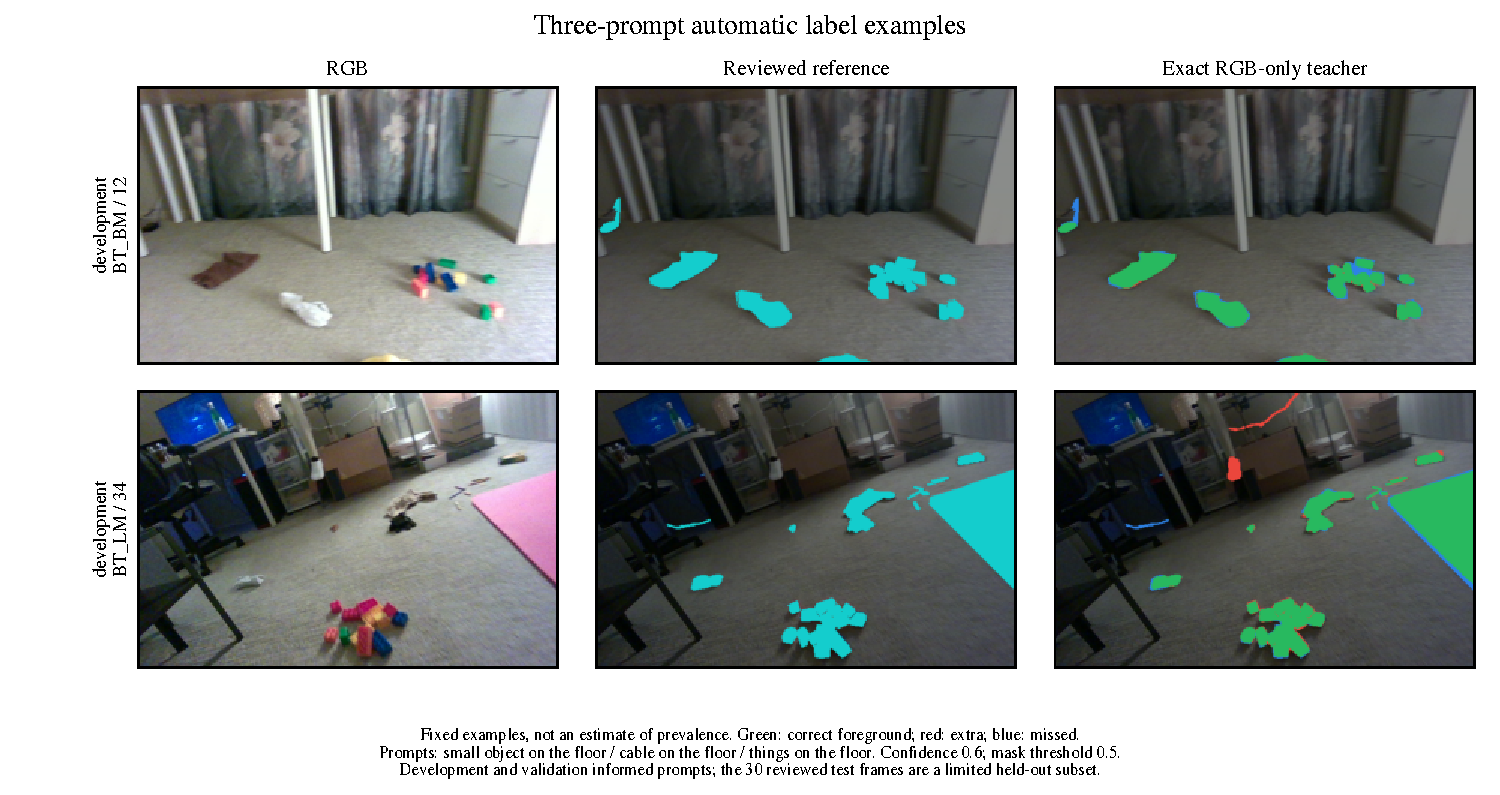
\includegraphics[width=0.91\textwidth,page=1]{figures/automatic_teacher_examples.pdf}
\includegraphics[width=0.91\textwidth,page=2]{figures/automatic_teacher_examples.pdf}
\caption{SAM 3 labels on two prompt-development and two validation frames next to the reviewed references. The examples show error types, not their frequency.}
\label{fig:teacher-devval}
\end{figure}

\clearpage
\section{Consistency Across Training Seeds}\label{app:seed-consistency}

Figure~\ref{fig:cloth-seeds} shows all three seeds. On the poster,
RGB-D seed 0 misses all cloths; seeds 1 and 2 find three. Every ESANet
version misses the flat white towel in all 15 observations. In seed 0,
D covers 99.85\% of the crumpled white tissue, but adjusted overlap is
0.428 because of surrounding predicted background.

\begin{figure}[!htbp]
\centering
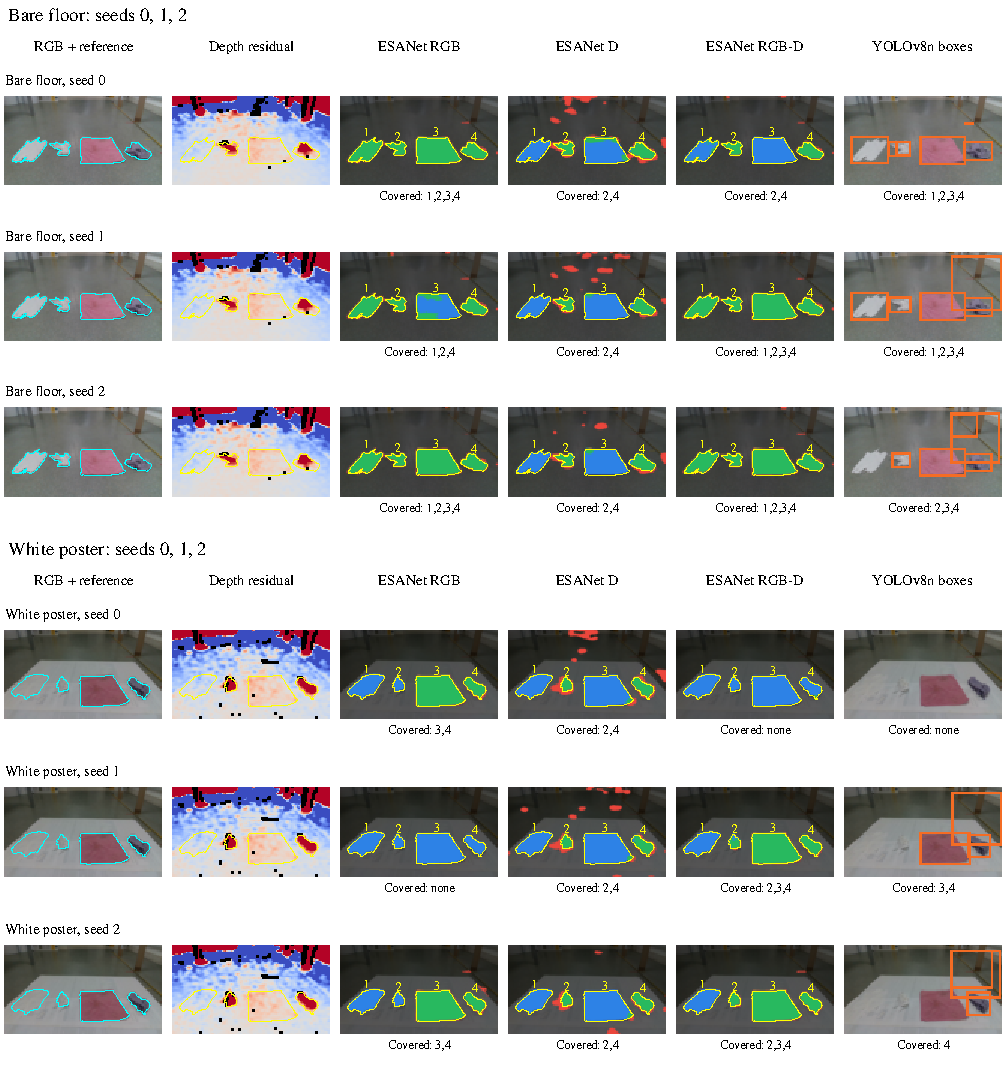
\includegraphics[width=0.92\textwidth]{figures/cloth_scenes_all_seeds.pdf}
\caption{All three seeds on the same two cloth scenes (frame 2). Bare-floor seeds 0/1/2 are grouped first, followed by poster seeds 0/1/2. IDs and colors follow Fig.~\ref{fig:cloth}; native YOLO boxes are orange. }
\label{fig:cloth-seeds}
\end{figure}
